\documentclass[journal]{IEEEtran}
\usepackage[english]{babel}

\usepackage{amssymb, amsmath} %Paquetes matemáticos de la American Mathematical 
\usepackage[utf8]{inputenc}
\usepackage{graphicx}
\usepackage{float}
\usepackage{hyperref}
\usepackage{listings}
\usepackage{xcolor}

\definecolor{codegreen}{rgb}{0,0.6,0}
\definecolor{codegray}{rgb}{0.5,0.5,0.5}
\definecolor{codepurple}{rgb}{0.58,0,0.82}
\definecolor{backcolour}{rgb}{0.95,0.95,0.92}
% Definicio de estilo para el codigo fuente que se cita
\lstdefinestyle{mystyle}{
    backgroundcolor=\color{backcolour},   
    commentstyle=\color{codegreen},
    keywordstyle=\color{magenta},
    numberstyle=\tiny\color{codegray},
    stringstyle=\color{codepurple},
    basicstyle=\ttfamily\footnotesize,
    breakatwhitespace=false,         
    breaklines=true,                 
    captionpos=b,                    
    keepspaces=true,
    numbers=left,                    
    numbersep=5pt,                  
    showspaces=false,                
    showstringspaces=false,
    showtabs=false,                  
    tabsize=2,
}
\lstset{style=mystyle}

\renewcommand{\lstlistingname}{Código}

\ifCLASSINFOpdf

\else

\fi
\begin{document}

\title{Ejercicio 3 - tema 7 \\ Administración de data files}
%
\author{Vicente Romero Andrade}

\markboth{Ejercicio 3 - tema 7 Administración de data files, Julio~2021}%
{Shell \MakeLowercase{\textit{et al.}}: }
% The only time the second header will appear is for the odd numbered pages

\maketitle


\IEEEpeerreviewmaketitle

\section{Objetivo}
% The very first letter is a 2 line initial drop letter followed

\IEEEPARstart{E}{l} objetivo es Poner en práctica las tareas de administración básicas 
que se asocian con el mantenimiento de data files: cambiar su ubicación, poner un data 
file fuera de línea, etc.

\section{Desarrollo}
\subsection{sentencias}
\begin{lstlisting}[language=sql, caption=s-00-crea-usuario.sql,label={lst:codigo1}]
connect sys/system2 as sysdba
CREATE USER VRA0602 IDENTIFIED BY VRA0602 quota unlimited on users;
GRANT CONNECT TO VRA0602;
GRANT CREATE TABLE TO VRA0602;
\end{lstlisting}
\begin{lstlisting}[language=sql, caption=s-01-crear-tabla.sql,label={lst:codigo2}]
whenever sqlerror exit rollback
set serveroutput on
connect VRA0602/VRA0602
-- B
declare
  v_count number;
  v_username varchar2(30) := 'VRA0602';
  v_table varchar2(30) := 'EMPLEADO';
begin
  --Verificar si la table existe
  select count(*) into v_count
  from all_tables
  where table_name = v_table
  and owner = v_username;
  --Si existe la tabla, entonces se borra
  if v_count > 0 then
    execute immediate 'drop table '||v_table;
  end if;
  execute immediate 'create table '||v_table||' (
    id number,
    nombre_completo varchar2(80) not null,
    num_cuenta varchar2(9),
    expediente clob,
    constraint pk_empleado primary key(id),
    constraint empleado_num_cuenta_uk unique(num_cuenta)
  )';
end;
/
insert into empleado(id,nombre_completo,num_cuenta,expediente) values (1,'Vicente Romero Andrade','312097792',null);
commit;
-- C
select 
        SEGMENT_NAME, 
        SEGMENT_TYPE, 
        TABLESPACE_NAME,
        BYTES,
        BLOCKS,
        EXTENTS 
    from USER_SEGMENTS 
        where SEGMENT_NAME like '%EMPLEADO%';
-- D
select
        SEGMENT_NAME,
        SEGMENT_TYPE,
        TABLESPACE_NAME,
        BYTES,
        BLOCKS,
        EXTENTS
    from USER_SEGMENTS
        where SEGMENT_NAME like '%EMPLEADO%'
          or SEGMENT_NAME in (select SEGMENT_NAME from USER_LOBS ul where ul.TABLE_NAME = 'EMPLEADO')
          or SEGMENT_NAME in (select INDEX_NAME from USER_LOBS ul where ul.TABLE_NAME = 'EMPLEADO');
whenever sqlerror continue
\end{lstlisting}
\begin{figure}[H]
  \centering
  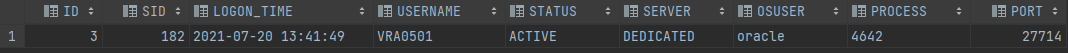
\includegraphics[scale=.22]{captura_1.png}
   \caption{Salida punto C}
   \label{fig:validador_1}
\end{figure}
\begin{figure}[H]
  \centering
  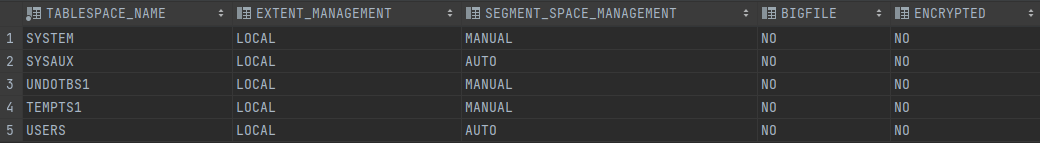
\includegraphics[scale=.22]{captura_2.png}
   \caption{Salida punto D}
   \label{fig:validador_2}
\end{figure}

\section{Conclusiones}
Se encontro una forma eficiente de consultar los segmentos creados en una tabla, 
el unico incoveniente es que estos dependen de que sean creados con el nombre de la tabla 
para su busqueda.
\ifCLASSOPTIONcaptionsoff
  \newpage

\fi

\end{document}
